% Name: Machine learning mind map
% Description: The three kinds of machine learning, supervised, unsupervised, and reinforcement, each with the tasks or methods that belong to it.
% Tags: mind map, machine learning, supervised learning, overview

\usetikzlibrary{mindmap}

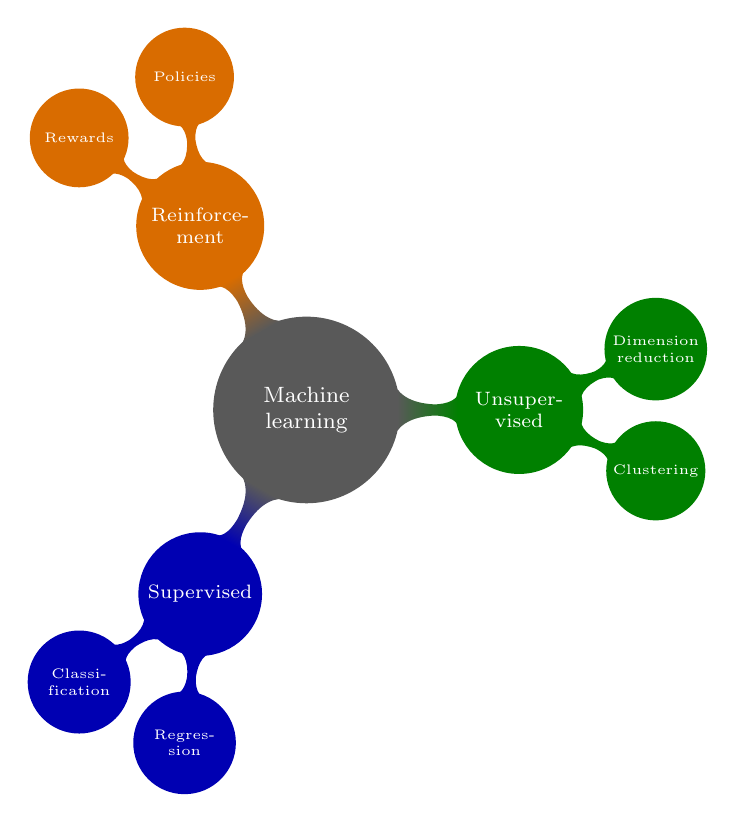
\begin{tikzpicture}[
  small mindmap, grow cyclic,
  every node/.style={concept, execute at begin node=\hskip0pt},
  concept color=gray!70!black, text=white,
  level 1/.append style={level distance=2.7cm, sibling angle=120},
  level 2/.append style={level distance=1.9cm, sibling angle=48},
]
  \node {Machine learning}
    child[concept color=blue!70!black] { node {Super\-vised}
      child { node {Classi\-fication} }
      child { node {Regres\-sion} }
    }
    child[concept color=green!50!black] { node {Unsuper\-vised}
      child { node {Cluster\-ing} }
      child { node {Dimen\-sion reduc\-tion} }
    }
    child[concept color=orange!85!black] { node {Reinforce\-ment}
      child { node {Policies} }
      child { node {Rewards} }
    };
\end{tikzpicture}
